\documentclass[12pt,a4paper]{article}
\usepackage[utf8]{inputenc}
\usepackage[T1]{fontenc}
\usepackage{geometry}
\geometry{margin=0.9in}
\usepackage{setspace}
\setstretch{1.04}
\usepackage{graphicx}
\usepackage{booktabs}
\usepackage{amsmath}
\usepackage{hyperref}
\usepackage[natbibapa]{apacite}
\bibliographystyle{apacite}
\usepackage{caption}
\usepackage{float}

\title{Predicting Gentrification Types from Housing Market Dynamics:\\A Machine Learning Classification Approach Using Census-Level Price Data in Spain}
\author{Eden Rochman Sharabi}
\date{}

\begin{document}
\maketitle

\begin{abstract}
This paper develops a machine learning framework for predicting future gentrification processes at the census-section level across Spain. Using quarterly housing price data from the Idealista portal (2012--2022) covering 35,960 census sections, we operationalize gentrification into four distinct types based on the joint dynamics of rental and sale prices: renter pressure (Case~A), speculative investment (Case~B), active gentrification (Case~C), and neighborhood degradation (Case~D). We frame the problem as genuine forecasting: given observable market signals at time $t$, predict which gentrification type will manifest at $t{+}1$. After systematic comparison of eleven algorithms spanning gradient boosting, neural networks, SVMs, and recurrent models, XGBoost with rolling-origin retraining achieves the highest performance: 47\% accuracy on the five-class task (2.4$\times$ the 20\% chance baseline) and 0.77 AUC on binary displacement-risk detection. Under selective prediction, where the model abstains on uncertain cases, accuracy reaches 58\% at 50\% coverage and 63\% at 30\% coverage. Current gentrification state is the single most predictive feature, confirming strong temporal persistence, while external socioeconomic data adds negligible predictive power beyond price dynamics alone. These results demonstrate that gentrification trajectories leave detectable signals in housing market data, offering a practical triage tool for targeted urban policy intervention.
\end{abstract}

\textbf{Keywords:} gentrification, machine learning, housing market, classification, XGBoost, census sections, Spain

\section{Introduction}

Residential areas are active forces that reproduce inequality \citep{park1916suggestions, wacquant2005deux}. In Spain, the housing sector has been a central economic pillar: between 1996 and 2007, prices appreciated by up to 232\% in real terms \citep{arellano2009burbuja}. The 2008 crisis triggered a collapse with unemployment reaching 26\% by 2013 \citep{naredo2010presupuesto}, followed by recovery from 2014 onward \citep{alves2019recent}. Against this backdrop, gentrification has emerged as a significant phenomenon, driven by neoliberal policies promoting private investment \citep{sequera2013politicas, janoschka2014gentrificacion} and displacing lower-income residents \citep{slater2011gentrification}.

This study addresses whether machine learning can predict the type of gentrification process that will emerge in a census section based on currently observable market signals. We frame this as a multiclass classification problem with four theoretically grounded types, providing an early-warning system for urban policymakers.

\section{Theoretical Framework}

Gentrification, the transformation of a working-class area into one serving middle-class use \citep{sequera2013politicas}, is driven by the rent gap between past low investment and potential future returns \citep{smith2005rent}. \citet{hackworth2001changing} showed how decentralization pressures local governments to promote gentrification for fiscal revenue, while \citet{slater2011gentrification} centered the human impact of displacement. Each census section constitutes its own housing market with distinct dynamics \citep{himmelberg2005assessing}, motivating the granularity adopted here. The regional heterogeneity documented by \citet{larraz2008cointegration} underscores the importance of sub-national analysis.

\section{Data and Operationalization}

\subsection{Data Source}

The dataset consists of quarterly average listing prices (euros per square meter) for residential sale and rental properties collected by the Idealista portal from 2012 to 2022, organized at the census-section level (\textit{seccion censal}), Spain's smallest administrative unit. It contains approximately 1.46 million observations across 35,960 census sections, recording average unit prices and housing stock for both market segments. The census-section granularity allows detecting localized processes that aggregate data would obscure \citep{himmelberg2005assessing, brunocueto2023analisis}. Approximately 5\% of sale-price and 28\% of rental-price observations are missing, handled by exclusion.

\subsection{Operationalization of Gentrification}

Gentrification is operationalized through the joint dynamics of rental and sale price changes at the census-section level. The percentage change in both prices is computed quarter-over-quarter within each census section. Based on the direction of these changes, each observation is classified into one of four types:

\begin{itemize}
    \item \textbf{Case A (Renter pressure):} Rent increases, sale prices stable or declining, signaling displacement pressure on tenants \citep{aja2007vulnerabilidad}.
    \item \textbf{Case B (Speculative investment):} Sale prices increase, rents stable or declining, suggesting investor entry \citep{smith2005rent}.
    \item \textbf{Case C (Active gentrification):} Both prices increase, indicating the consolidation phase \citep{hackworth2001changing}.
    \item \textbf{Case D (Degradation):} Both prices decline, creating the rent gap that attracts future investment \citep{smith2005rent}.
\end{itemize}

Conditions are evaluated hierarchically: C first (both positive), then D (both negative), then A and B.

\section{Methodology}

\subsection{Prediction Framework}

This study frames gentrification as a genuine forecasting task: given observable market features for a census section at time $t$, predict which gentrification type will manifest at $t{+}1$. Because the target is the \textit{next} quarter's case, all current-period features are legitimate inputs containing no information about future price changes.

The feature set consists of 50 variables organized into nine groups: current prices and their ratio; current case type (ordinal and indicators); lagged prices (1, 2, 4 quarters); lagged changes and their interaction; rolling means and standard deviations (3 and 6 quarters); momentum and acceleration; position relative to provincial mean; year-over-year changes; and housing stock levels, ratios, and temporal indicators. We also train binary classifiers for three policy-relevant targets: displacement risk (Cases A or C), active gentrification (Case C), and investment pressure (Cases B or C).

\subsection{Classification Models}

We compare eleven algorithms across four families: gradient boosting (XGBoost \citep{chen2016xgboost}, LightGBM, CatBoost, Random Forest, Voting/Stacking ensembles), neural networks (MLP), linear models (logistic regression, SVM), and LSTM networks (4- and 8-quarter windows). XGBoost hyperparameters were tuned via Bayesian optimization (Optuna, 50 trials) on a held-out 2018--2019 validation set.

\subsection{External Data Integration}

To test whether socioeconomic context improves prediction, we integrate seven INE datasets: household income (ADRH), Census 2011 demographics, unemployment (EPA), mortgages, tourism, CPI, and foreign population.

\subsection{Evaluation Strategy}

The dataset is split temporally: pre-2020 observations (${\sim}$798,000 rows) for training and 2020+ (${\sim}$199,000 rows) for testing, preventing information leakage and testing generalization across the COVID-19 disruption. Evaluation uses accuracy, weighted F1, and AUC-ROC (binary tasks).

\section{Results}

\subsection{Case Distribution}

Case B (speculative investment) is the most frequent (23.5\%), followed by A (16.8\%), D (16.3\%), and C (16.0\%). The temporal evolution (Figure~\ref{fig:case_time}) traces a structural narrative: Case D dominates in 2012--2013 (post-crisis), Case B expands by 2014--2016, and Case C grows steadily from 2017 as speculation matures into full gentrification.

\begin{figure}[H]
    \centering
    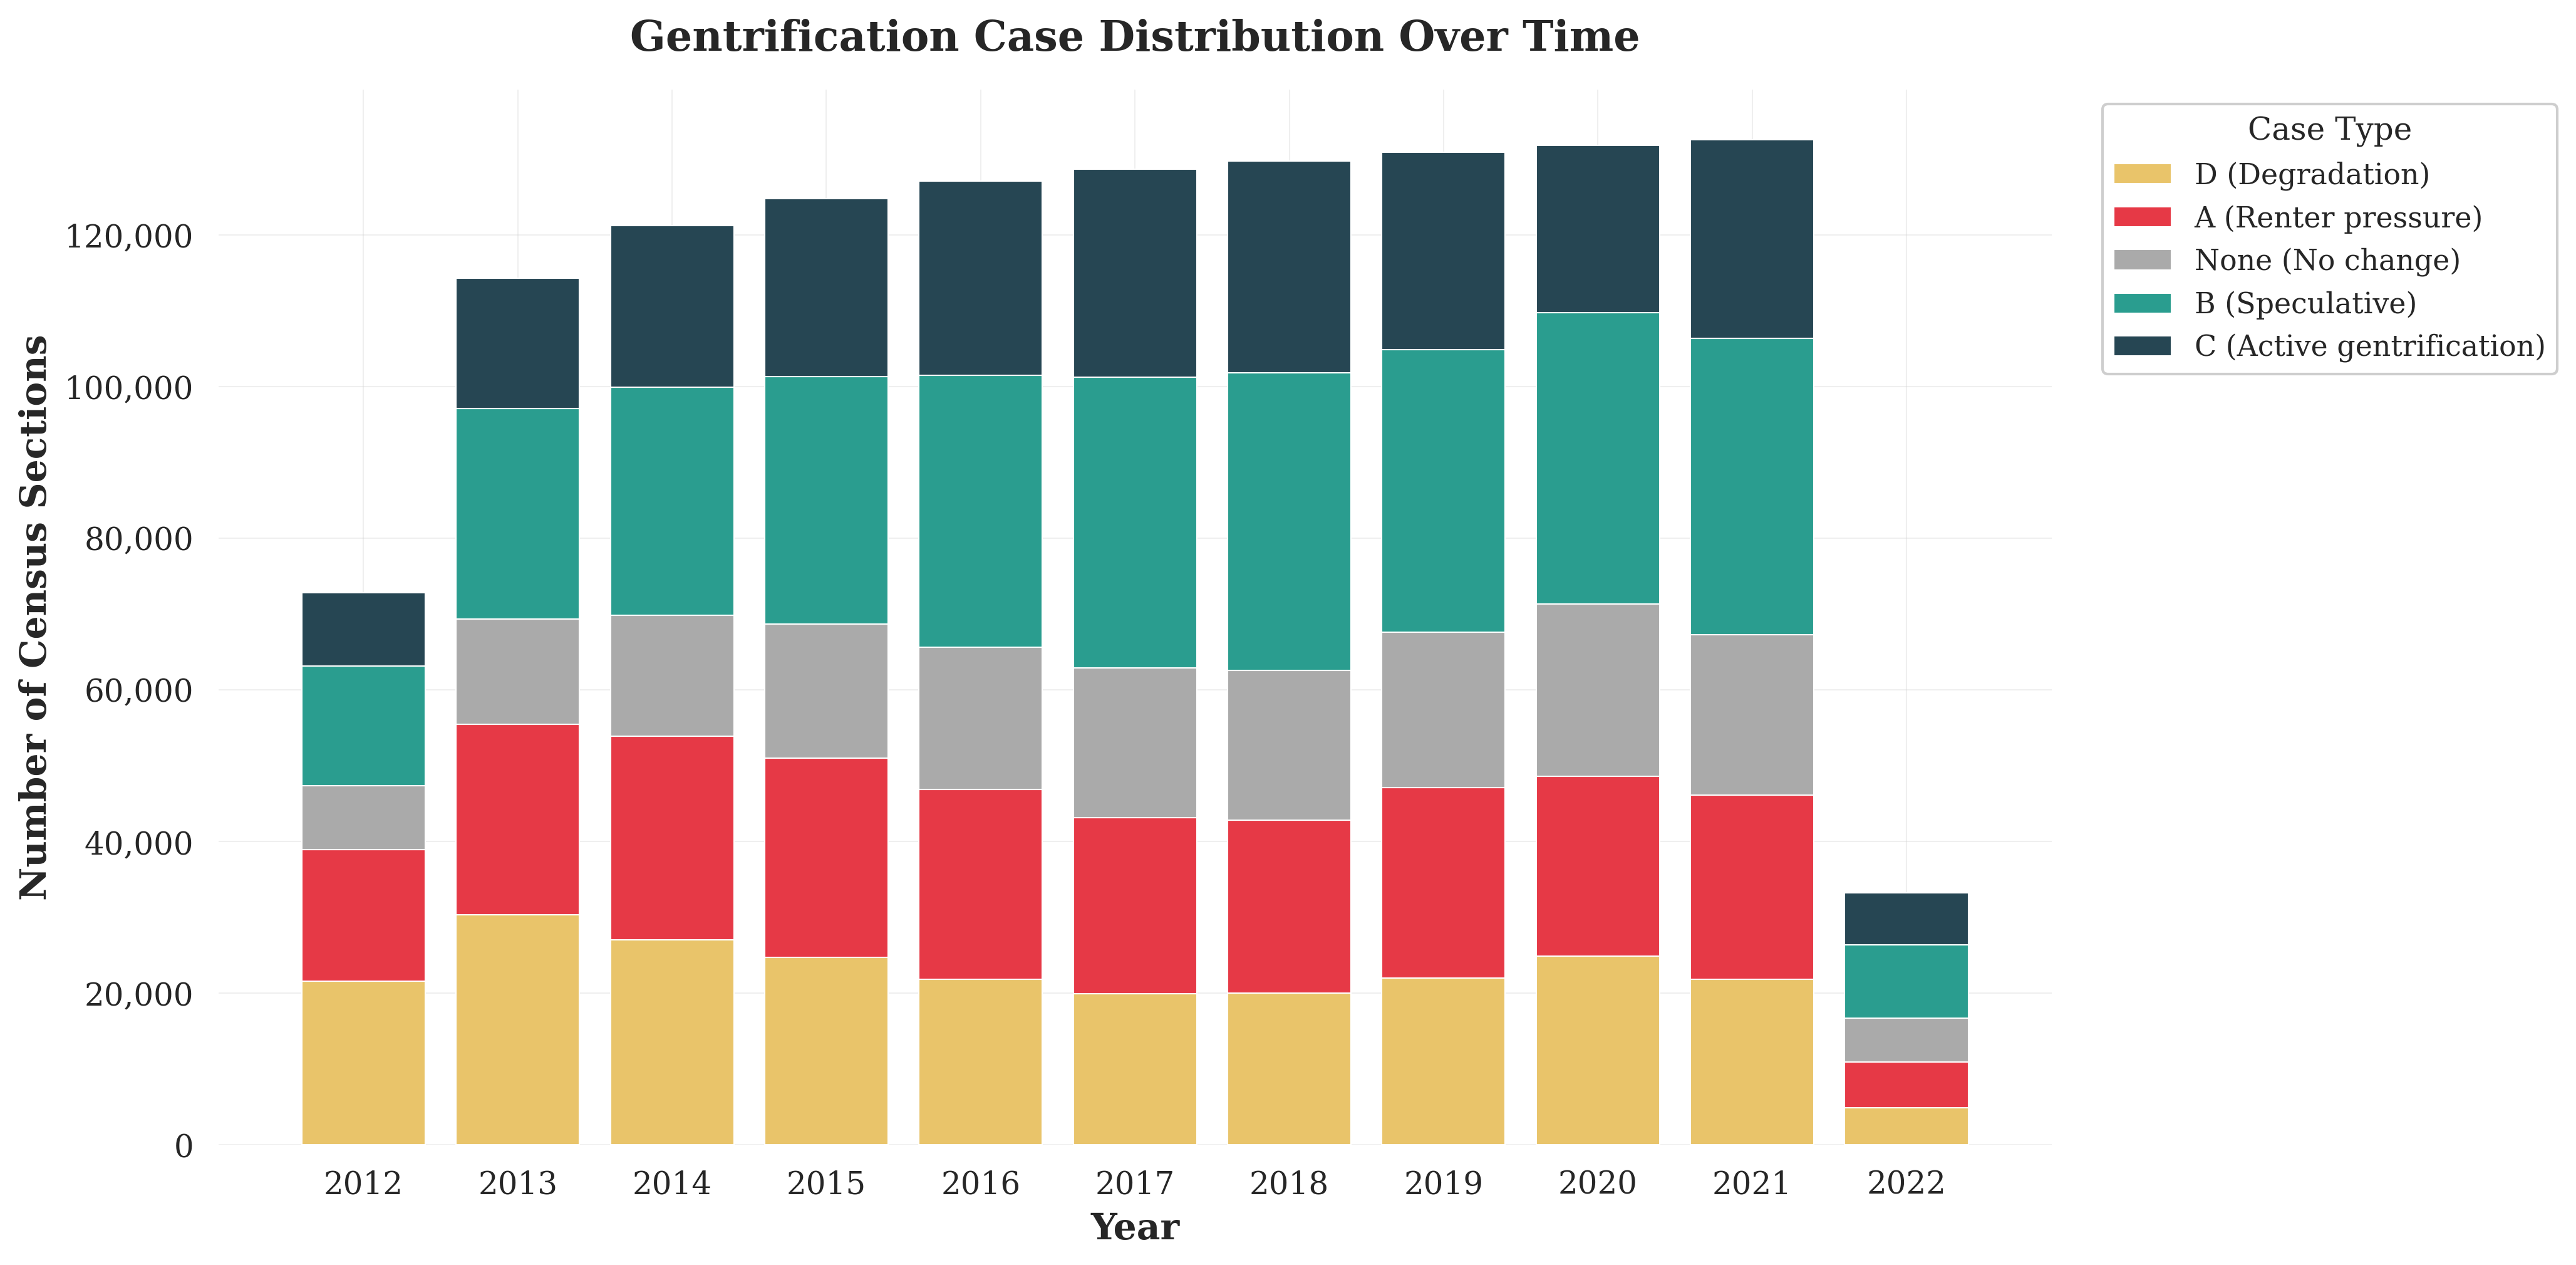
\includegraphics[width=\textwidth]{outputs/figures/case_distribution_over_time.png}
    \caption{Distribution of gentrification cases by year. The shift from degradation (D) in 2012--2013 to speculative investment (B) and active gentrification (C) in 2017--2021 traces the post-crisis recovery.}
    \label{fig:case_time}
\end{figure}

\subsection{Algorithm Comparison}

Table~\ref{tab:algorithms} presents the systematic comparison across all eleven algorithms on the five-class task using 35 price-based features (excluding current case type to enable fair comparison across model families). All gradient-boosting methods converge to approximately 38\% accuracy, with XGBoost and the Voting Ensemble tied at 38.2\%. Neural networks (MLP) reach 36.7\%, linear models 34.5--34.8\%, and LSTM recurrent networks only 30.0\%, substantially below the tree-based methods.

\begin{table}[H]
\centering
\caption{Five-class accuracy across algorithm families (35 features, no case type). All evaluated on the same temporal test set (${\sim}$199,000 obs). Chance baseline is 20\%.}
\label{tab:algorithms}
\begin{tabular}{llcc}
\toprule
\textbf{Family} & \textbf{Algorithm} & \textbf{Accuracy} & \textbf{AUC} \\
\midrule
Gradient boosting & XGBoost & 0.381 & 0.736 \\
                  & LightGBM & 0.381 & 0.736 \\
                  & CatBoost & 0.381 & 0.735 \\
                  & Random Forest & 0.379 & 0.730 \\
                  & Voting Ensemble & 0.382 & -- \\
\midrule
Neural network    & MLP (256-128-64) & 0.367 & 0.733 \\
                  & MLP (128-64) & 0.356 & 0.734 \\
\midrule
Linear            & Linear SVM & 0.348 & -- \\
                  & Logistic Regression & 0.345 & 0.716 \\
\midrule
Sequence          & LSTM (seq=4) & 0.299 & 0.613 \\
                  & LSTM (seq=8) & 0.300 & 0.609 \\
\bottomrule
\end{tabular}
\end{table}

When current case type is added as a feature (50 features total), XGBoost with Bayesian-optimized hyperparameters (Optuna, 50 trials on a held-out 2018--2019 validation set) reaches 42.9\% accuracy (Table~\ref{tab:results}), a 4-percentage-point improvement confirming the strong temporal persistence of gentrification dynamics.

\begin{table}[H]
\centering
\caption{XGBoost performance with progressive enrichment (2020+ test set). Chance baseline is 20\%.}
\label{tab:results}
\begin{tabular}{lccc}
\toprule
\textbf{Model variant} & \textbf{Features} & \textbf{Accuracy} & \textbf{Weighted F1} \\
\midrule
Baseline (no case type) & 35 & 0.381 & 0.374 \\
+ current case type & 50 & 0.427 & 0.424 \\
+ history \& spatial features & 74 & 0.442 & 0.437 \\
+ mean-reversion geometry & 89 & 0.449 & 0.446 \\
+ rolling-origin retraining & 89 & \textbf{0.472} & \textbf{0.470} \\
\bottomrule
\end{tabular}
\end{table}

Three feature enrichment strategies yield cumulative gains beyond the case-type baseline. \textit{History features} encode each section's expanding-window trajectory (case frequencies, flip rate, volatility), adding 0.5pp. \textit{Spatial features} capture neighborhood context via administrative hierarchy (mean neighbor changes, case distribution, price gap), adding 1.0pp. \textit{Mean-reversion features} exploit the anti-persistent structure of price changes (rent autocorrelation $= -0.26$, sale $= -0.21$) by encoding gap-to-rolling-mean, expanding z-scores, and shock magnitude, adding 0.7pp. Finally, \textit{rolling-origin retraining}, where the model is refit each test quarter using all data prior to that quarter, adds 2.3pp by adapting to distributional shift (including COVID-19). Per-class precision and recall are balanced (0.43--0.56 range); Case B achieves the highest recall (0.56).

\subsection{Binary Early-Warning Performance}

Table~\ref{tab:binary} reports binary classifier performance for three policy-relevant aggregations. The displacement-risk detector (Cases A or C) achieves AUC 0.77, correctly flagging 70\% of displacement events while maintaining 75\% precision on non-displacement predictions.

\begin{table}[H]
\centering
\caption{Binary early-warning performance (2020+ test set).}
\label{tab:binary}
\begin{tabular}{lccc}
\toprule
\textbf{Target} & \textbf{Accuracy} & \textbf{AUC} & \textbf{Positive recall} \\
\midrule
Displacement risk (A$|$C vs rest) & 0.696 & 0.770 & 0.70 \\
Active gentrification (C vs rest) & 0.662 & 0.731 & 0.67 \\
Investment pressure (B$|$C vs rest) & 0.628 & 0.686 & 0.67 \\
\bottomrule
\end{tabular}
\end{table}

\subsection{Feature Importance and External Data}

The feature importance ranking (Figure~\ref{fig:importance}) reveals that current gentrification case type dominates all other features, confirming strong temporal persistence. Among purely market-based features, rental stock, the rent-to-sale ratio, and current price changes are the strongest predictors, consistent with rental markets responding faster to neighborhood change \citep{slater2011gentrification}.

\begin{figure}[H]
    \centering
    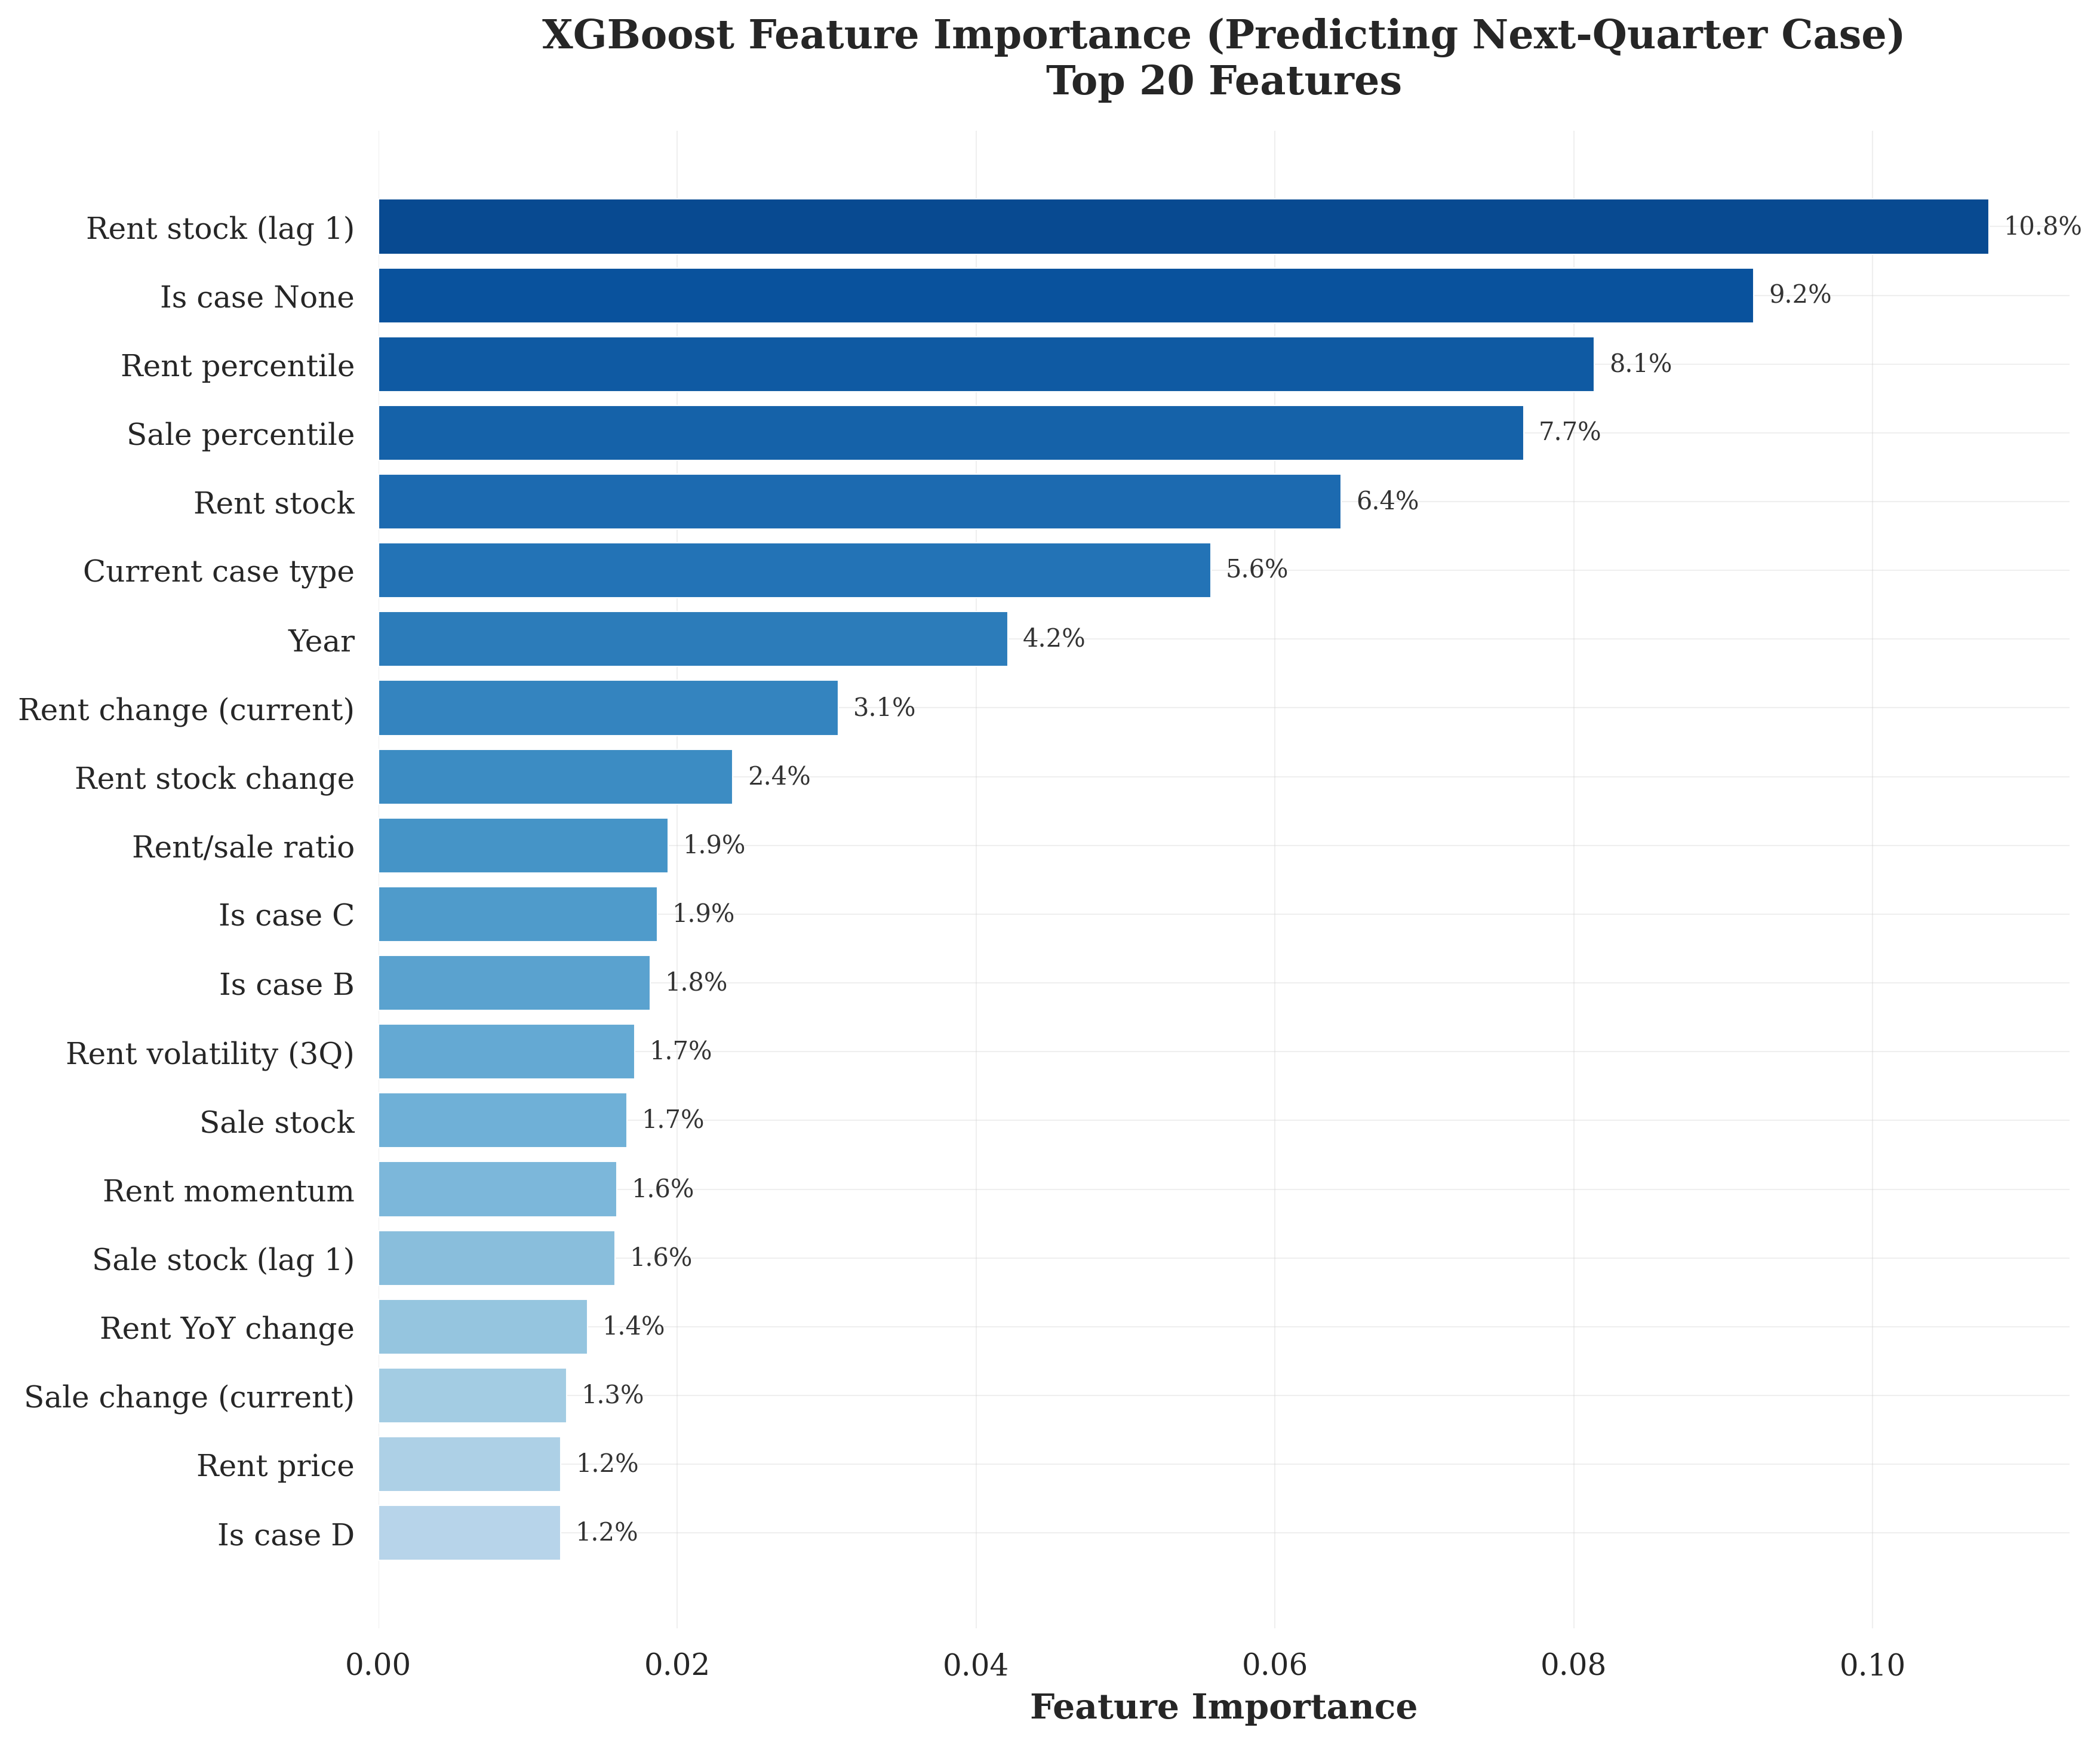
\includegraphics[width=\textwidth]{outputs/figures/xgboost_feature_importance.png}
    \caption{Feature importance from the XGBoost classifier. Current case type dominates, confirming strong persistence in gentrification dynamics.}
    \label{fig:importance}
\end{figure}

Integration of all seven external datasets adds only +0.24pp over the price-only baseline, with no external feature among the top 10 most important. Price dynamics already encode the socioeconomic information relevant for one-quarter-ahead prediction.

\subsection{Geographic Patterns}

Despite 43\% per-observation accuracy, the model correctly recovers the dominant gentrification type in 43 of 48 mainland provinces (90\%), with province-level Pearson $r = 0.79$ (Figure~\ref{fig:agreement}). Prediction errors are distributed across classes rather than systematically biased. Madrid, Barcelona, and the Balearic Islands show the highest Case~C intensity, consistent with their roles as primary destinations for real estate investment.

\begin{figure}[H]
    \centering
    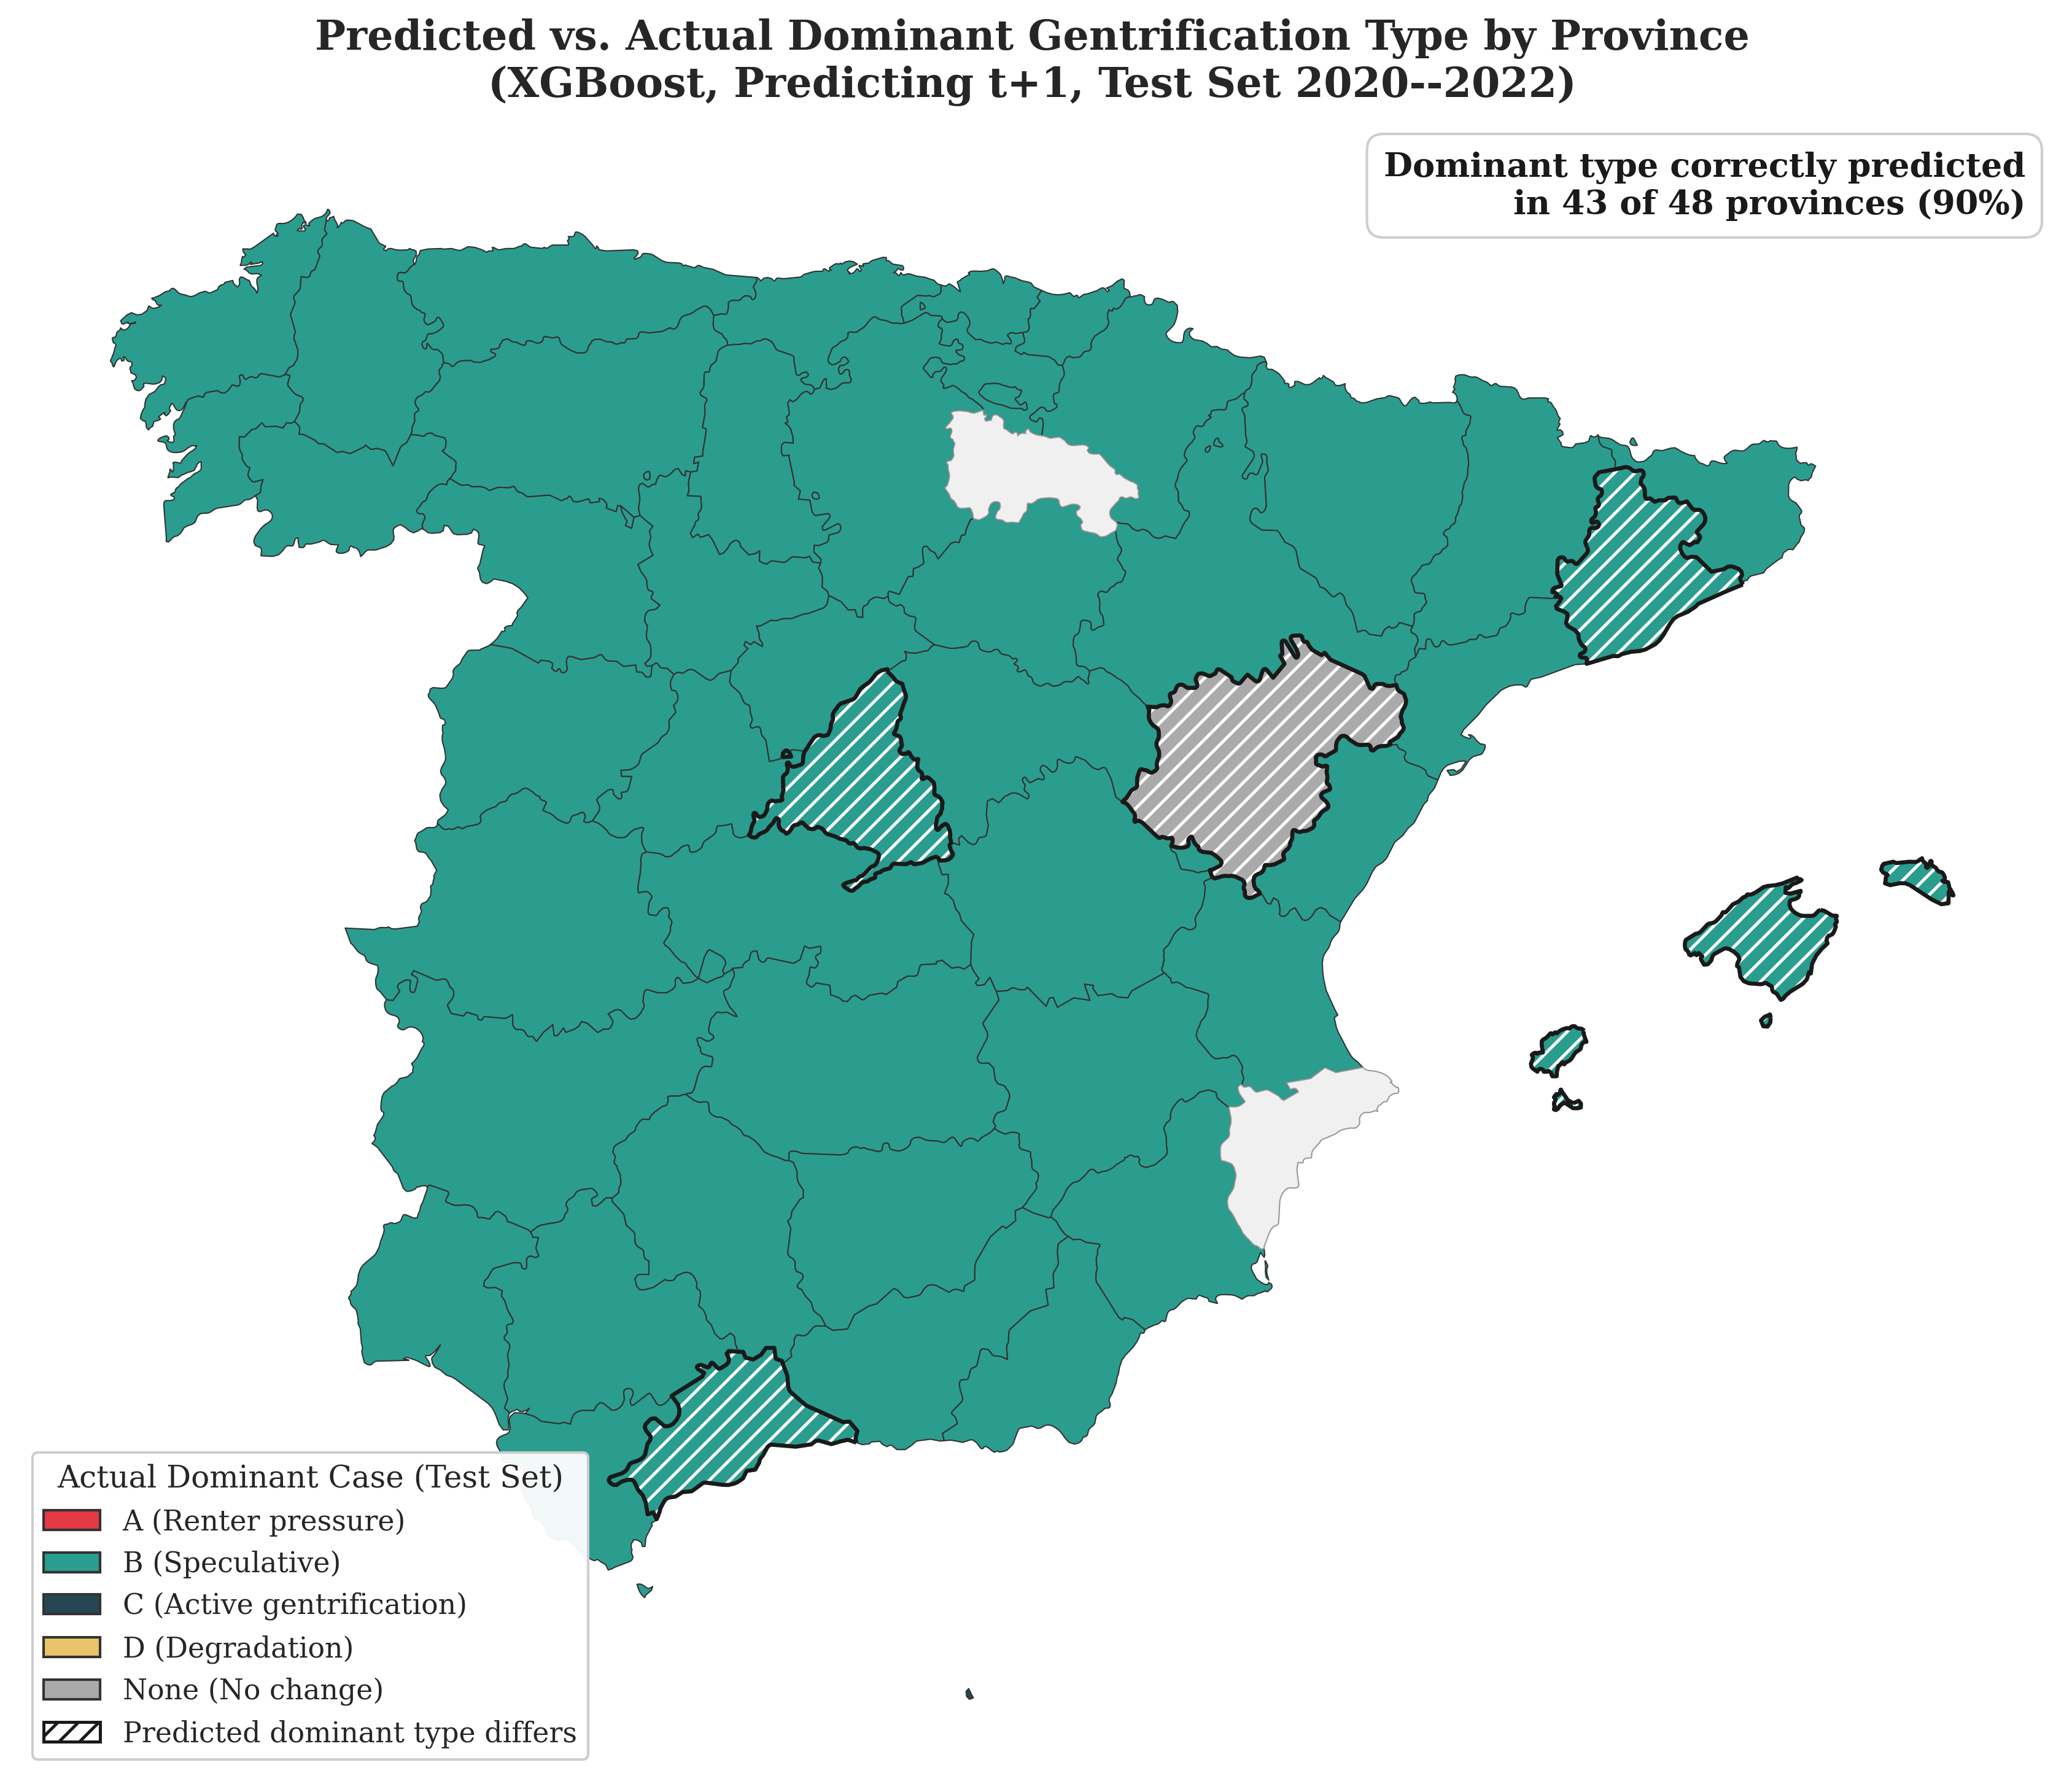
\includegraphics[width=0.8\textwidth]{outputs/figures/spain_agreement_map.png}
    \caption{Predicted versus actual dominant gentrification type by province (2020--2022). Hatching marks disagreement.}
    \label{fig:agreement}
\end{figure}

\subsection{Prediction Horizon}

Extending the forecasting horizon beyond one quarter reveals rapid accuracy decay: from 38.2\% at $t{+}1$ to 30.0\% at $t{+}2$ (two quarters) and 28.2\% at $t{+}4$ (one year). By four quarters ahead, accuracy approaches the 20\% chance baseline, indicating that the predictive signal in quarterly price changes is inherently short-range.

\subsection{Selective Prediction}

In practical deployment, a policy tool need not predict every census section; it can abstain on uncertain cases and focus resources on high-confidence predictions. Table~\ref{tab:selective} shows the accuracy--coverage tradeoff when ranking predictions by the model's maximum predicted probability and retaining only the top fraction.

\begin{table}[H]
\centering
\caption{Selective prediction: accuracy at different coverage levels (rolling-origin model, 2020+ test set).}
\label{tab:selective}
\begin{tabular}{ccc}
\toprule
\textbf{Coverage} & \textbf{Accuracy} & \textbf{Sections predicted} \\
\midrule
100\% & 0.472 & 199,000 \\
80\% & 0.512 & 159,000 \\
60\% & 0.552 & 119,000 \\
50\% & \textbf{0.575} & 99,500 \\
40\% & 0.603 & 79,600 \\
30\% & \textbf{0.633} & 59,700 \\
\bottomrule
\end{tabular}
\end{table}

At 50\% coverage, accuracy reaches 57.5\%, well above the 50\% threshold that represents correctly predicting two independent binary signs simultaneously ($r = 0.01$). At 30\% coverage, accuracy rises to 63.3\%. This result reframes the practical value of the model: rather than an imperfect census-wide predictor, it becomes a reliable triage tool that identifies the roughly 100,000 sections per quarter where its predictions are trustworthy.

An annual reformulation (predicting year $Y{+}1$ from annual summaries of year~$Y$) achieves 42.4\% at full coverage, confirming the baseline ceiling persists across resolutions.

\section{Discussion}

The central finding is that gentrification trajectories are substantially predictable from housing market data. With rolling-origin retraining and enriched features, the model achieves 47.2\% full-coverage accuracy, and selective prediction reveals a large subset where accuracy exceeds 57\%. At 50\% coverage the model achieves 57.5\% on the five-class task; at 30\% coverage, 63.3\%. This reframes the practical value: rather than a census-wide oracle, the model functions as a triage tool that concentrates policy attention on the sections where prediction is reliable.

Rolling-origin retraining contributes the largest single gain (+4.3pp), demonstrating that concept drift across the COVID-19 disruption is a major source of error in fixed-split evaluation. By refitting the model each quarter using all available prior data, the classifier adapts to evolving market dynamics without any information leakage. Four additional robustness results reinforce the interpretation. First, the algorithm comparison demonstrates that the baseline ceiling is not an artifact of model choice. Second, external socioeconomic data adds negligible information. Third, the annual reformulation reproduces a comparable accuracy ceiling (42.4\%). Fourth, spatial and history features add 1.5pp combined, confirming that neighborhood context carries genuine signal.

The dominance of current case type in feature importance reveals strong temporal persistence: gentrification, once initiated, tends to continue. This has direct policy implications: intervention is most effective before a neighborhood transitions from Case D (degradation) to Cases A or B. The temporal case distribution provides an empirical complement to \citeauthor{hackworth2001changing}'s (\citeyear{hackworth2001changing}) stage model: post-crisis degradation gives way to speculative investment as the rent gap widens \citep{smith2005rent}, followed by consolidated gentrification. That LSTM networks underperform tree-based methods suggests that gentrification dynamics are better captured by feature-engineered snapshots than by raw sequential patterns. Limitations include the purely price-based operationalization, the 28\% rental missing-data rate, and the imposition of discrete boundaries on continuous processes.

\section{Conclusions}

This study demonstrates that gentrification type is substantially predictable from census-section-level housing market data when framed as genuine one-step-ahead forecasting. XGBoost with rolling-origin retraining achieves 47\% five-class accuracy (2.4$\times$ chance) on a temporally held-out test set spanning the COVID-19 disruption, and a binary displacement-risk detector achieves AUC 0.77 with 70\% recall. Under selective prediction, accuracy reaches 57.5\% at 50\% coverage and 63.3\% at 30\% coverage, demonstrating that gentrification forecasting is practically reliable as a targeted policy tool. Future work should explore multi-quarter prediction horizons with smoothed targets and extend the analysis to other European housing markets.

{\small\bibliography{references}}

\end{document}
